\section{Restrospettiva}
Durante lo sviluppo di questo progetto il team ha lavorato seguendo un processo
di svuluppo SCRUM-inspired, come consigliato nelle regole del progetto.
In particolare, sono stati effettuati cinque sprint della durata di circa una 
settimana ciascuno. All'inizio e alla fine di ogni sprint il team si è riunito
per discutere i task completati nello sprint precedente e per pianificare i task
dello sprint successivo. È stato utilizzato un foglio di calcolo condiviso per
tenere traccia delle attività tramite un product backlog e degli sprint backlog.
Per ciascuno sprint backlog è stata utilizzata una tabella riempita con le attività 
principali da completare, ciascuna suddivisa in task più piccoli, associati a un
responsabile e a una stima del tempo necessario per il completamento. Durante la settimana 
dedicata allo sprint, sempre tramite lo stesso foglio di calcolo, ciascun membro
del team ha tenuto traccia del tempo realmente impiegato per completare ciascun 
task. Alla fine di ogni sprint la tabella è stata poi inserita nella repository
del progetto come documento di retrospettiva dello sprint.

Questa tipologia di organizzazione si è rivelata molto utile per l'organizzazione
del lavoro e la coordinazione. L'identificazione chiara e continuativa degli obiettivi
da raggiungere ha permesso di ottenere risultati tangibili in tempi brevi e
di avere una visione chiara del progresso del progetto nonché della quantità
di tempo dedicato da ciascun membro del team. 

Di seguito vengono riportati il product backlog (figura \ref{fig:product-backlog}) e gli sprint backlog utilizzati durante lo sviluppo
insieme a un commento sui risultati ottenuti per ciascuno sprint.

\begin{figure}[ht!]
    \centering
    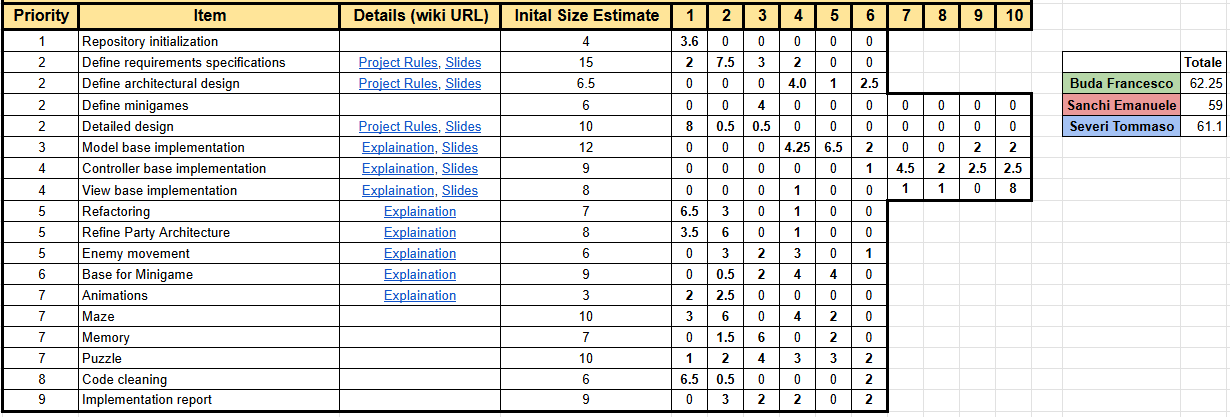
\includegraphics[width=1\textwidth]{figures/product-backlog.png}
    \caption{Product Backlog}
    \label{fig:product-backlog}
\end{figure}

\subsection{Sprint-1} \label{sec:sprint-1}
Il primo sprint (figura \ref{fig:backlog-sprint-1}) è stato dedicato alla definizione dei requisiti
e del design architetturale del progetto, oltre che alla creazione della repository e della struttura 
di base.
\begin{figure}[ht!]
    \centering
    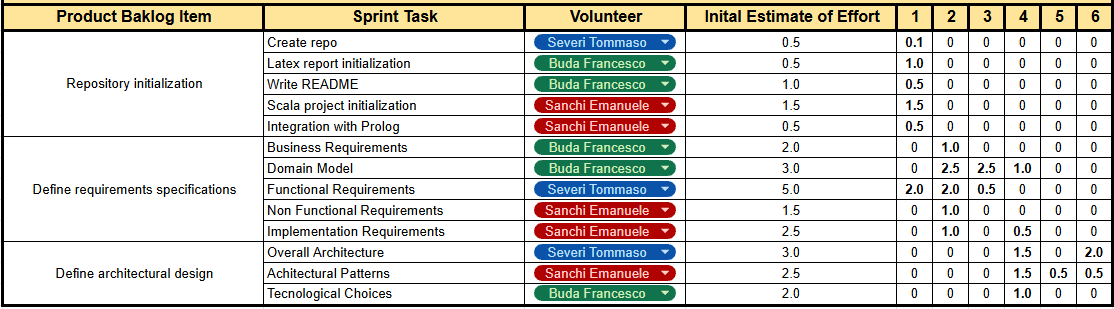
\includegraphics[width=1\textwidth]{figures/backlog-sprint-1.png}
    \caption{Backlog per lo Sprint-1}
    \label{fig:backlog-sprint-1}
\end{figure}
\subsection{Sprint-2} \label{sec:sprint-2}
Il secondo sprint (figura \ref{fig:backlog-sprint-2}) ha portato alla definizione dei minigiochi 
e del design di dettaglio, nonché alla realizzazione di una prima versione funzionante dell'applicazione, 
questa prima versione aveva le seguenti caratteristiche:
\begin{itemize}
    \item Schermata iniziale di Start
    \item Schermata di gioco principale
    \item Movimento del giocatore tramite frecce
    \item Movimento randomico del nemico
    \item Schermata di Game Over
\end{itemize}
\begin{figure}[ht!]
    \centering
    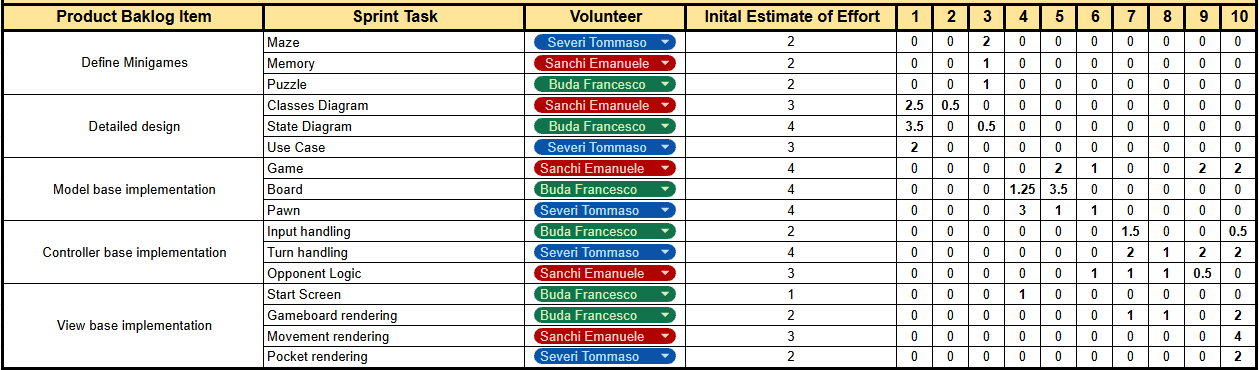
\includegraphics[width=1\textwidth]{figures/backlog-sprint-2.png}
    \caption{Backlog per lo Sprint-2}
    \label{fig:backlog-sprint-2}
\end{figure}
\subsection{Sprint-3} \label{sec:sprint-3}
Il terzo sprint (figura \ref{fig:backlog-sprint-3}) ha segnato il completamento delle funzionalità del
gioco principale e ha posto le basi per l'integrazione dei minigiochi. le funzionalità aggiunte sono state:
\begin{itemize}
    \item tiro di dadi iniziale per decidere il primo giocatore
    \item movimento intelligente del nemico
    \item rigenerazione del tabellone di gioco
    \item doppio tiro di dado per il vincitore di un minigioco
\end{itemize}
\begin{figure}[ht!]
    \centering
    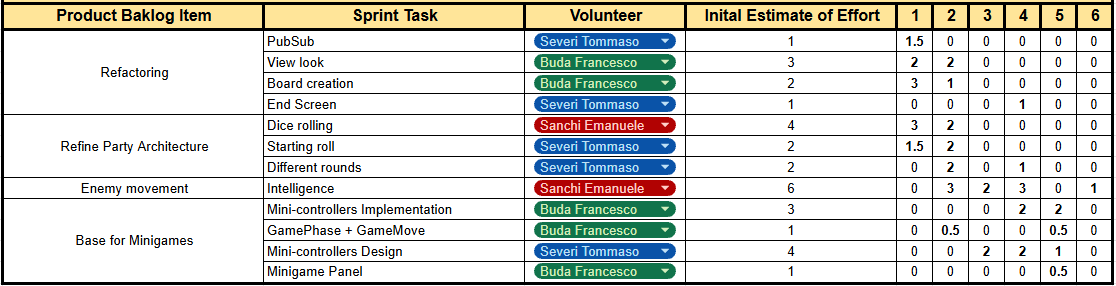
\includegraphics[width=1\textwidth]{figures/backlog-sprint-3.png}
    \caption{Backlog per lo Sprint-3}
    \label{fig:backlog-sprint-3}
\end{figure}
\subsection{Sprint-4} \label{sec:sprint-4}
Il quarto sprint (figura \ref{fig:backlog-sprint-4}) ha aggiunto al gioco principale delle semplici animazioni
e ha completato l'integrazione dei minigiochi maze, memory e puzzle.
\begin{figure}[ht!]
    \centering
    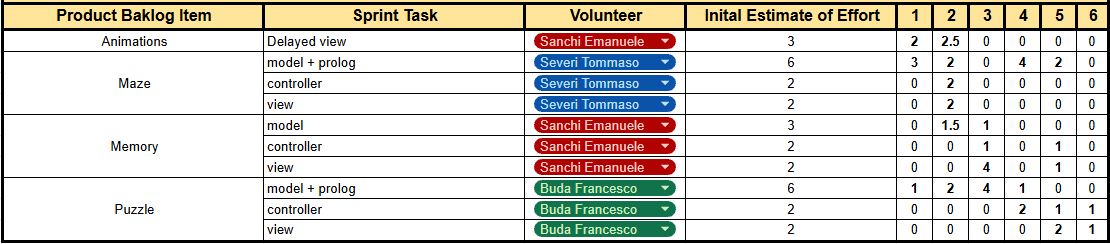
\includegraphics[width=1\textwidth]{figures/backlog-sprint-4.png}
    \caption{Backlog per lo Sprint-4}
    \label{fig:backlog-sprint-4}
\end{figure}
\subsection{Sprint-5} \label{sec:sprint-5}
Lo sprint-5 è stato lo sprint conclusivo del progetto, è stato dedicato alla pulizia del codice e al completamento della documentazione
e della relazione finale.

\begin{figure}[ht!]
    \centering
    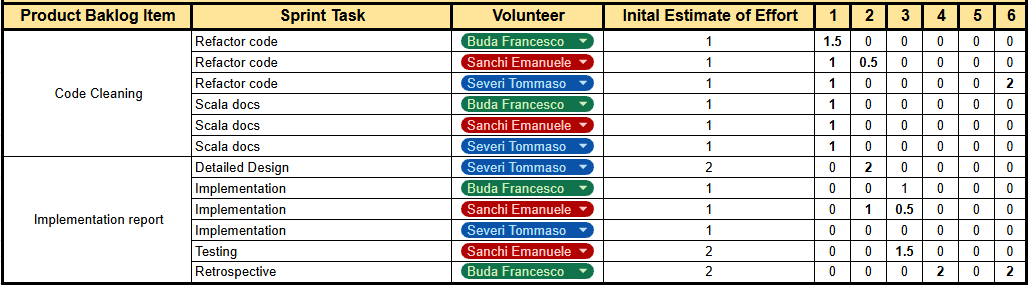
\includegraphics[width=1\textwidth]{figures/backlog-sprint-5.png}
    \caption{Backlog per lo Sprint-5}
    \label{fig:backlog-sprint-5}
\end{figure}